\documentclass[a4paper,11pt]{article} %indique la classe du document, et les options

%le pr\'eambule
\usepackage[english]{babel}
\usepackage{graphicx}
\usepackage{array}
\usepackage{multicol}
\usepackage{fancyhdr}
\usepackage{listings}
\setlength{\headheight}{15.2pt}
\pagestyle{fancy}
\selectlanguage{english}


%Titre
\makeatletter
\def\maketitle{

	\begin{multicols}{2}
		{\begin{center}
		{\LARGE \@title}\\
		\rule{3cm}{1pt}
	\end{center}}
		\begin{flushright}
			{\includegraphics[width=0.5\linewidth]{../../../Newcastle-University.jpg}}\\
			{\@date}\\
		\end{flushright}
	\end{multicols}	
	\vspace{1cm}
}
\def\email#1{\def\@email{#1}}
\makeatother
\email{nicolas.desfeux@gmail.com}
\date{\today}
\author{Nicolas Desfeux}
\title{
{Coursework 2\\Building a Total Order service
}}

\renewcommand{\thesection}{\textnormal{\Roman{section}})} 
\renewcommand{\thesubsection}{~~\textnormal{\alph{subsection}})} 
%document principal 

\begin{document}
\maketitle
\lhead{Nicolas Desfeux}
\rhead{Student No :110477367 - Erasmus student}
The purpose of this document is to show the system we design to provide a Total Order Service (TOS).
\section{Conditions and assumptions}
\subsection{Conditions}
The service have to satisfies the following three conditions : 
\begin{itemize}
\item (C1) Say messages m and m' are sent to process p. If sending of
m happened before sending of m', then the delivery of m to p
must happen before the delivery of m' to p.
( respects "happened before")
\item (C2) Say messages m and m' are sent to processes p and q. The
delivery of m to p happens before the delivery of m' to p if and
only if the delivery of m to q happens before the delivery of m'
to q (provides identical order)
\item (C3) any message sent to process p is eventually delivered to p.
(liveness)
\end{itemize}
\subsection{Assumptions}
\begin{itemize}
\item (A1) Processes have no access to synchronized physical clocks;
\item (A2) The communication subsystem guarantees that a sent
message is eventually delivered to the destination, but no bound
on transmission delays;
\item (A3) For any two processes p and q, messages sent by p to q are
received in the sent order;
\item (A4) Sending of a message to one or more destinations is a single
event within the sending process and,
\item (A5) Processes never crash and are uniquely ordered; this
ordering is known to each process.
\end{itemize}
\section{Building a Total Service Order}
Here is the system we are designing : \\
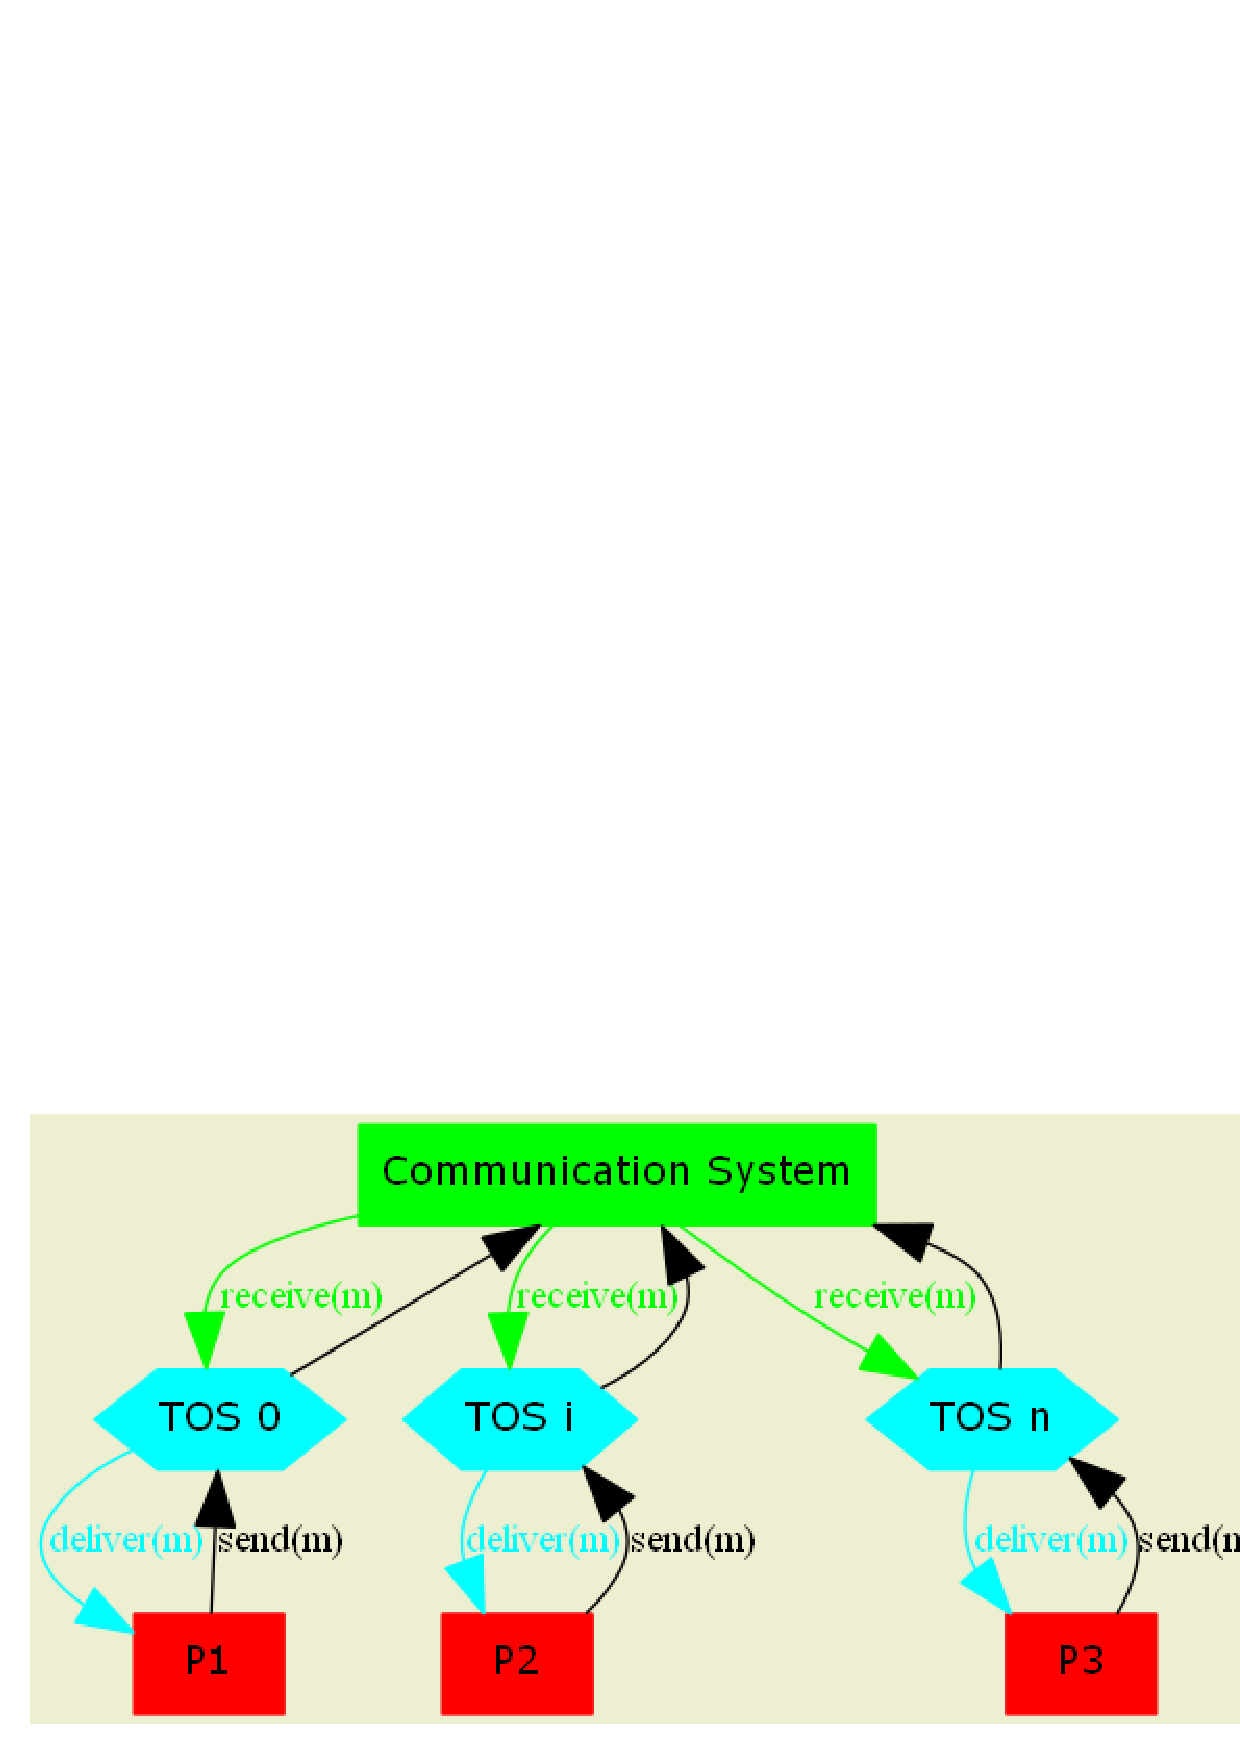
\includegraphics[scale=0.6]{design.png}
We're now going to focus on those three functions : 
\begin{itemize}
\item send(m) : What TOSi should do with m ?
\item receive(m) : How TOSi should handle m ?
\item deliver(m) : When TOSi should deliver a receive message m ?
\end{itemize}We are assuming that each TOS have access to a logical clock.
Here is the way it works: 
\renewcommand{\labelenumi}{(\roman{enumi})}
\renewcommand{\labelenumii}{(\alph{enumii})}
\begin{enumerate}
\item A process P send a message : it also adds the timestamp,  the destination(s) (process identifier) of the message, and the list of messages' timestamp not acknowledged by the destination TOS. then it adds to the list : the timestamp and the destination.
\item A TOS receive a message : We put it in a waiting list. Several cases can occurs : 
\begin{enumerate}
\item if the destination list included in the message is not empty, and the process is not the first in the list, put the message in a waiting list.
\item if the list of messages' timestamp not acknowledged by the destination process included in the message is empty : the TOS send an acknowledgment to the every process (contening the timestamp from the original message, the sender identifier, and the time stamp of the TOS which have been acknowledged), and deliver the message to the process. 
\item if the list of messages' timestamp not acknowledged by the destination process included in the message is not empty : The process put the message in a waiting list. 
\end{enumerate}
\item When a TOS receive a acknowledgment from a process : 
If the TOS is the TOS who send the original message :  it remove from it list of messages' timestamp no acknowledged by the destination process the correspondent timestamp and destination couple. \\After each message receive, the receiving TOS looks a this own list, to see if some messages can now by read. When they are readable, they are removed from the list, and read. 
Otherwise : if one message from the same sender is in it list : Check it destination list, if the TOS who's sending the ack. is in, removed it. If the list is empty, read the message. Else, don't deliver the message.
\end{enumerate}

\end{document}